\begin{figure*}
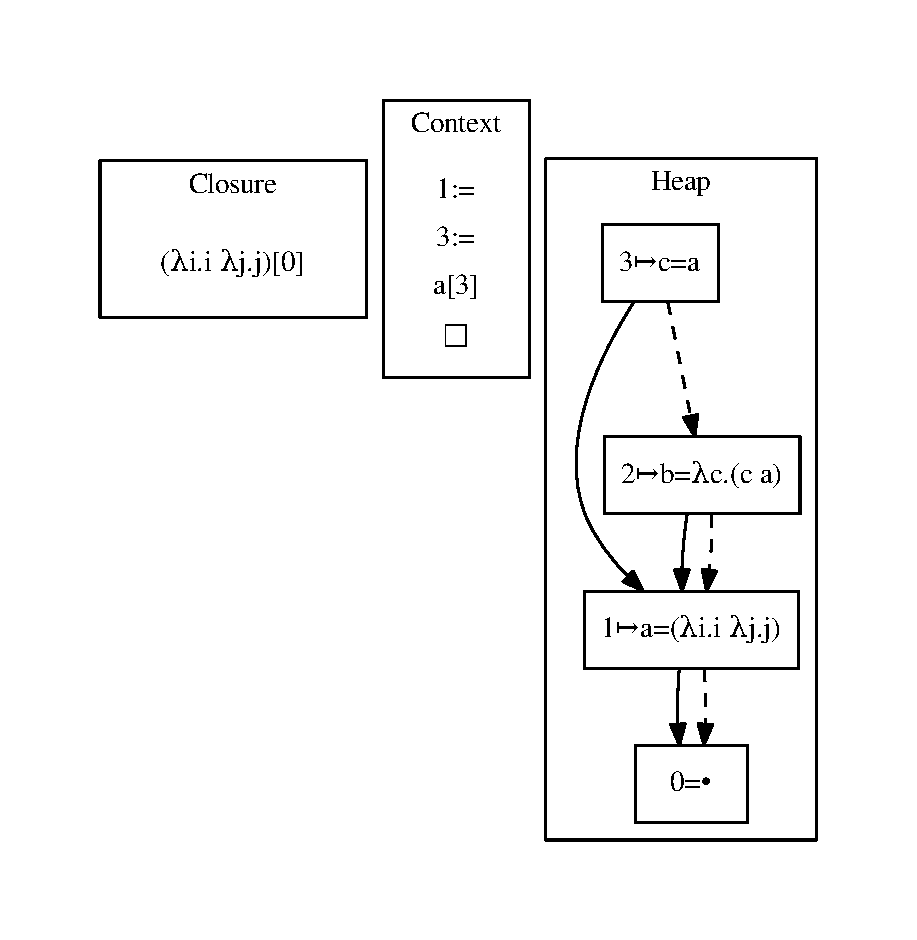
\includegraphics[width=\linewidth/3]{figures/12.pdf}
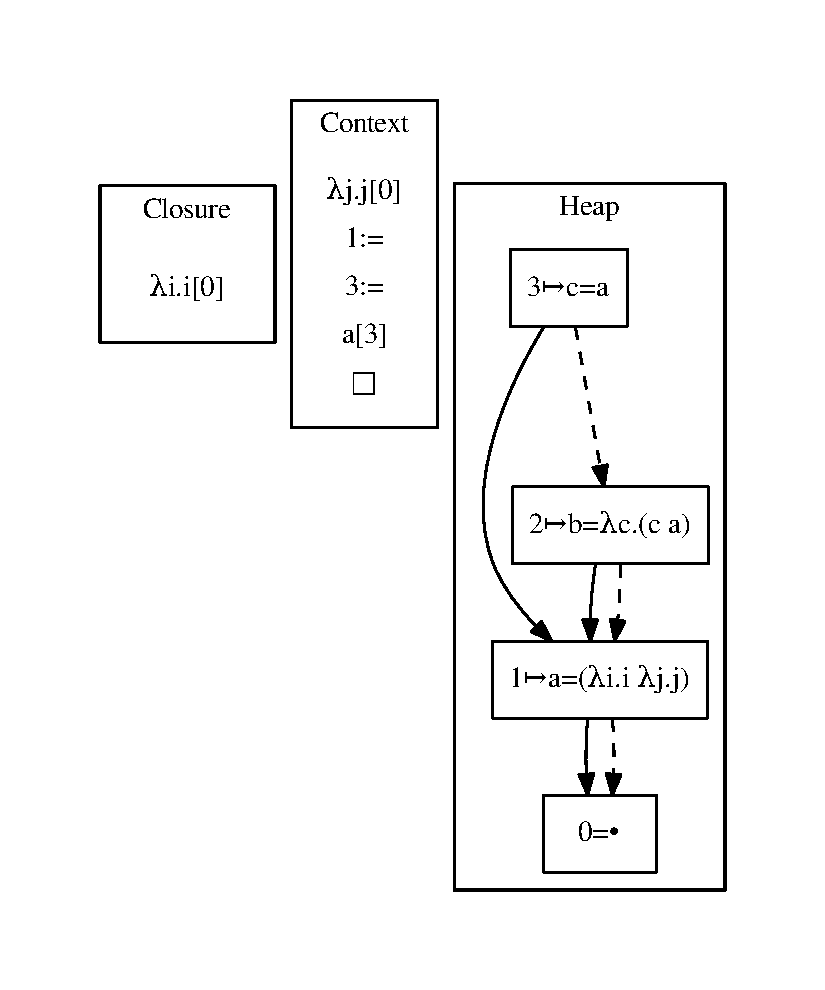
\includegraphics[width=\linewidth/3]{figures/13.pdf}
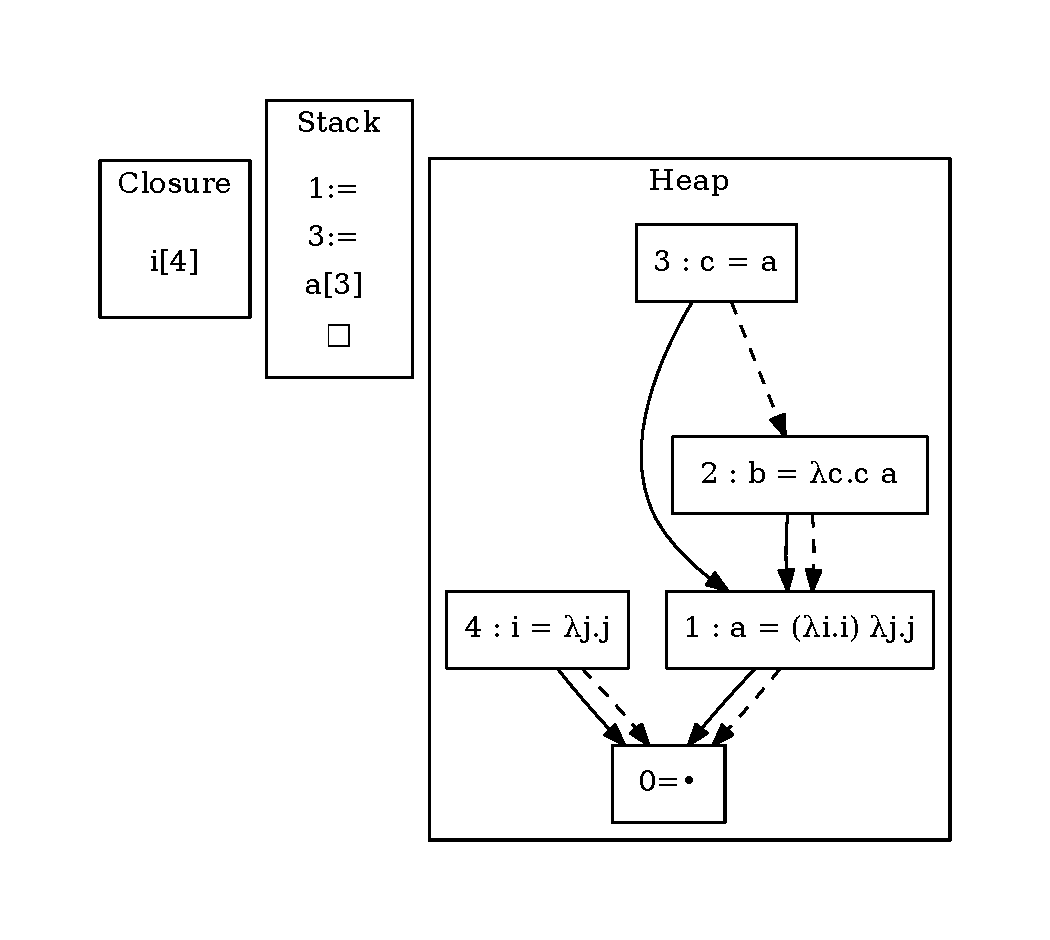
\includegraphics[width=\linewidth/3]{figures/14.pdf}
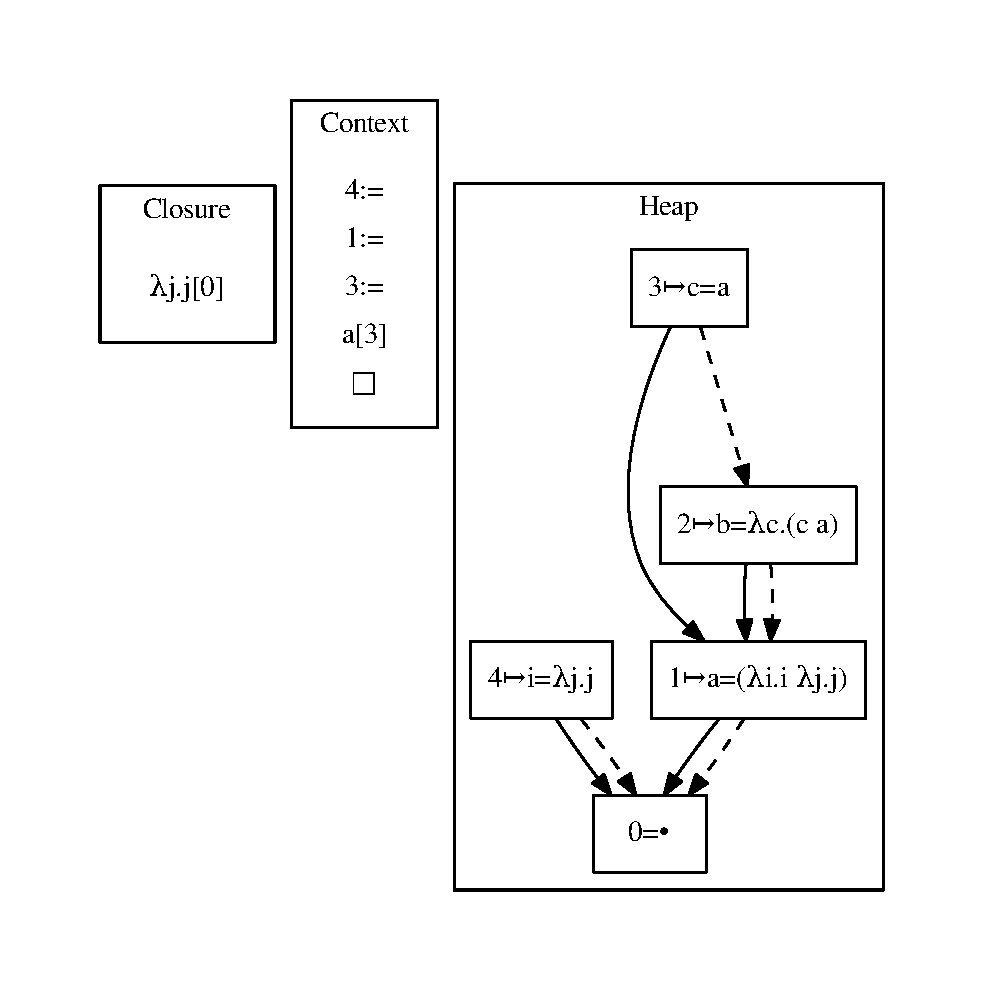
\includegraphics[width=\linewidth/3]{figures/15.pdf}
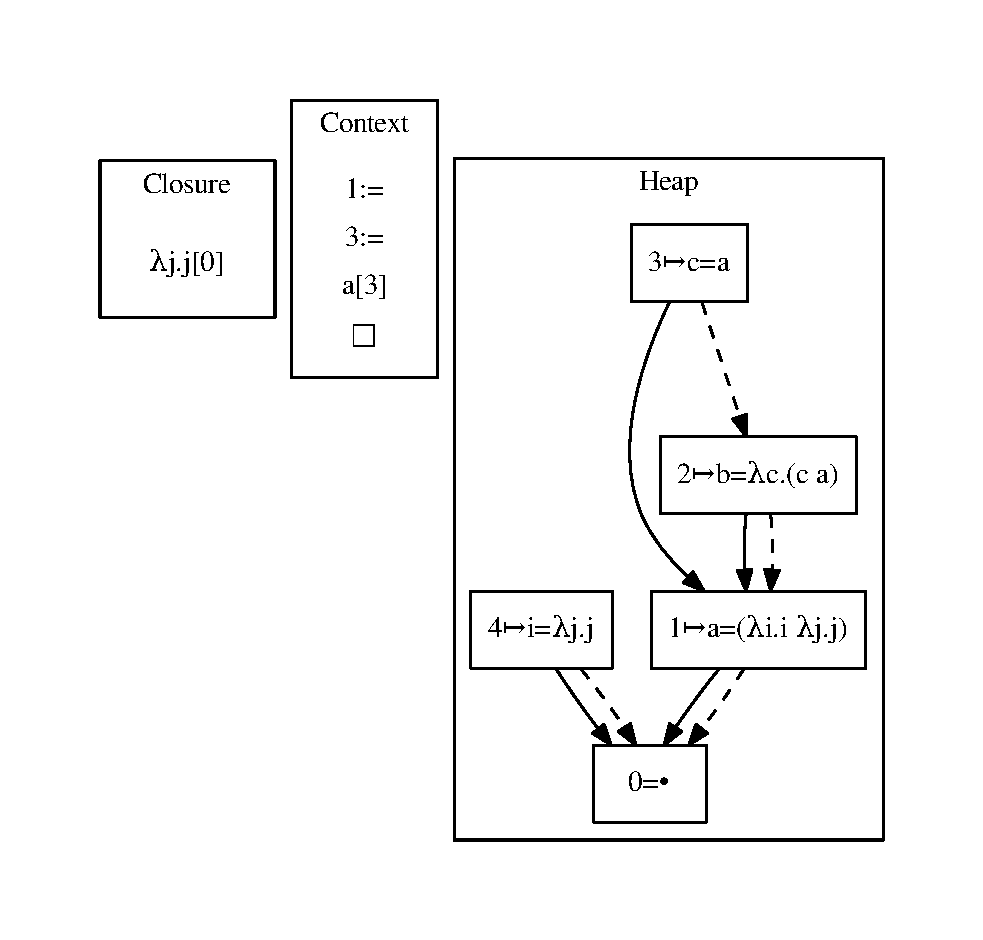
\includegraphics[width=\linewidth/3]{figures/16.pdf}
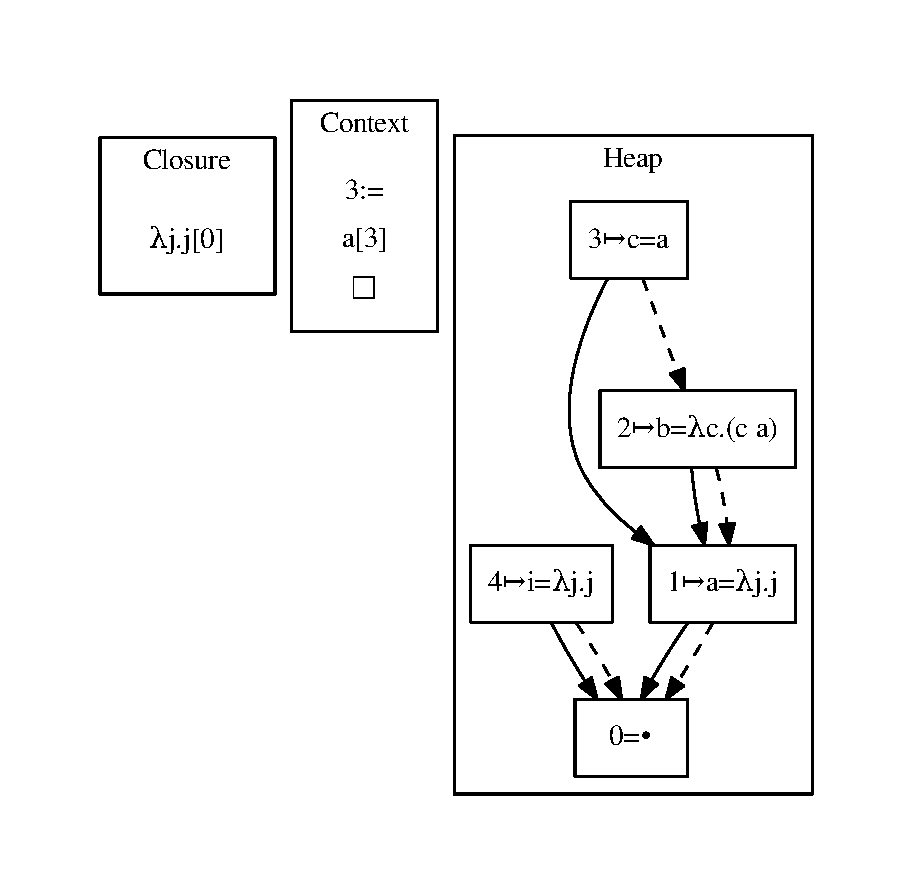
\includegraphics[width=\linewidth/3]{figures/17.pdf}
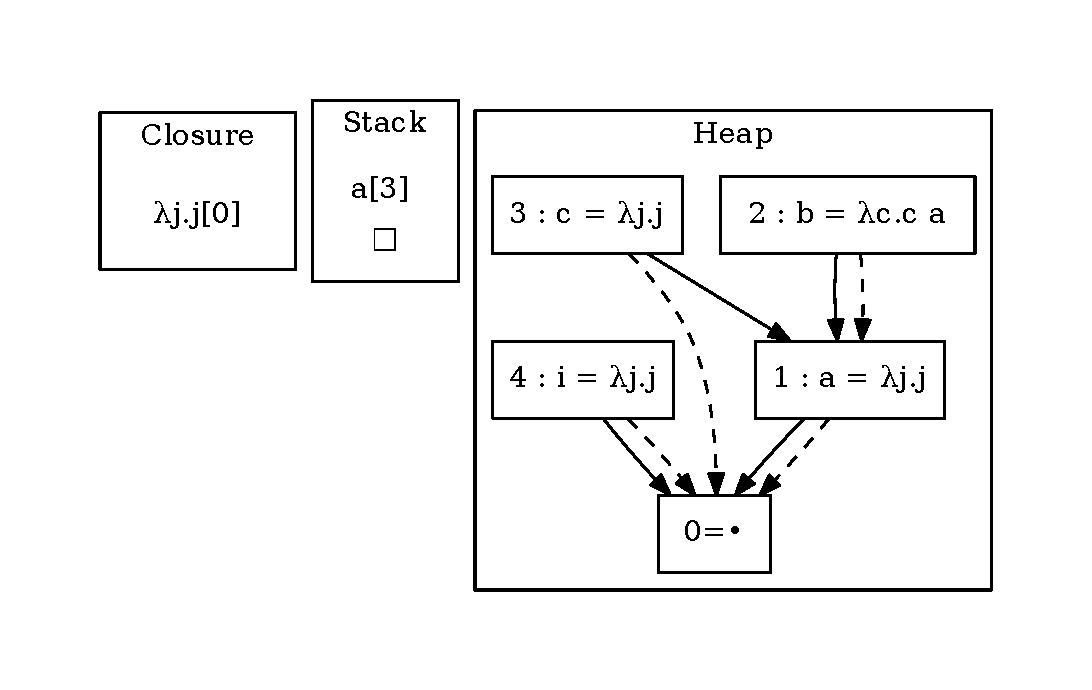
\includegraphics[width=\linewidth/3]{figures/18.pdf}
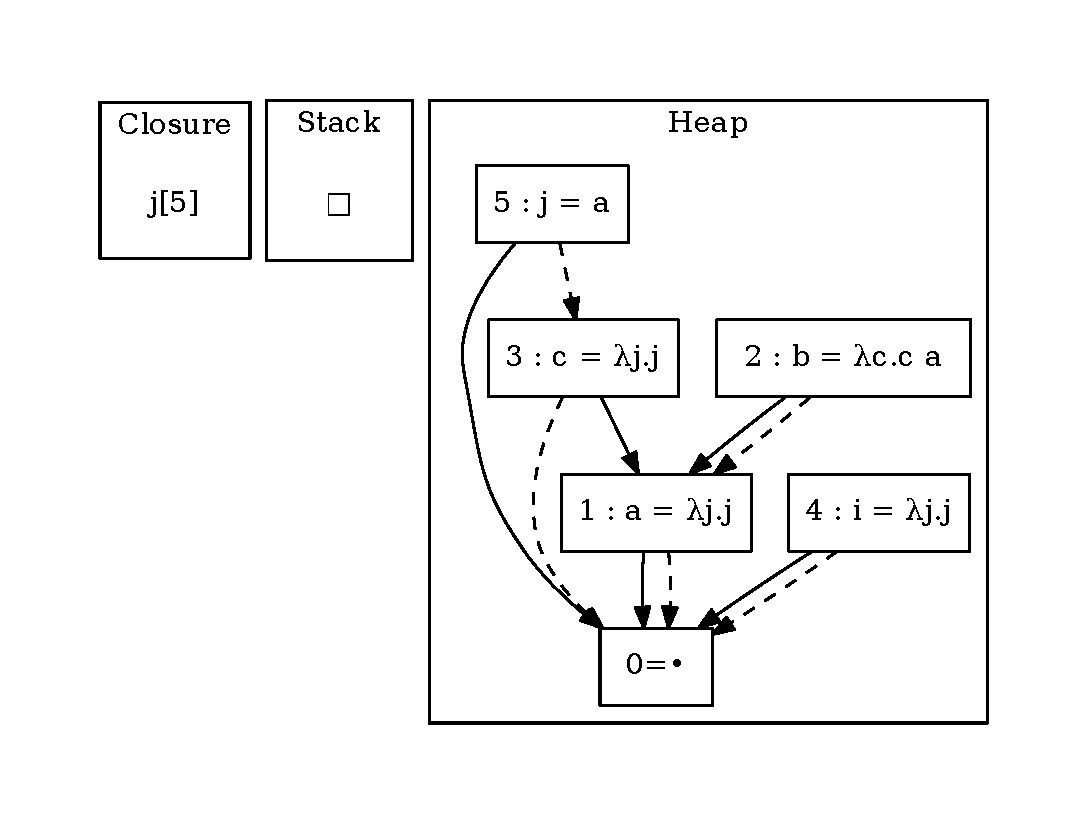
\includegraphics[width=\linewidth/3]{figures/19.pdf}
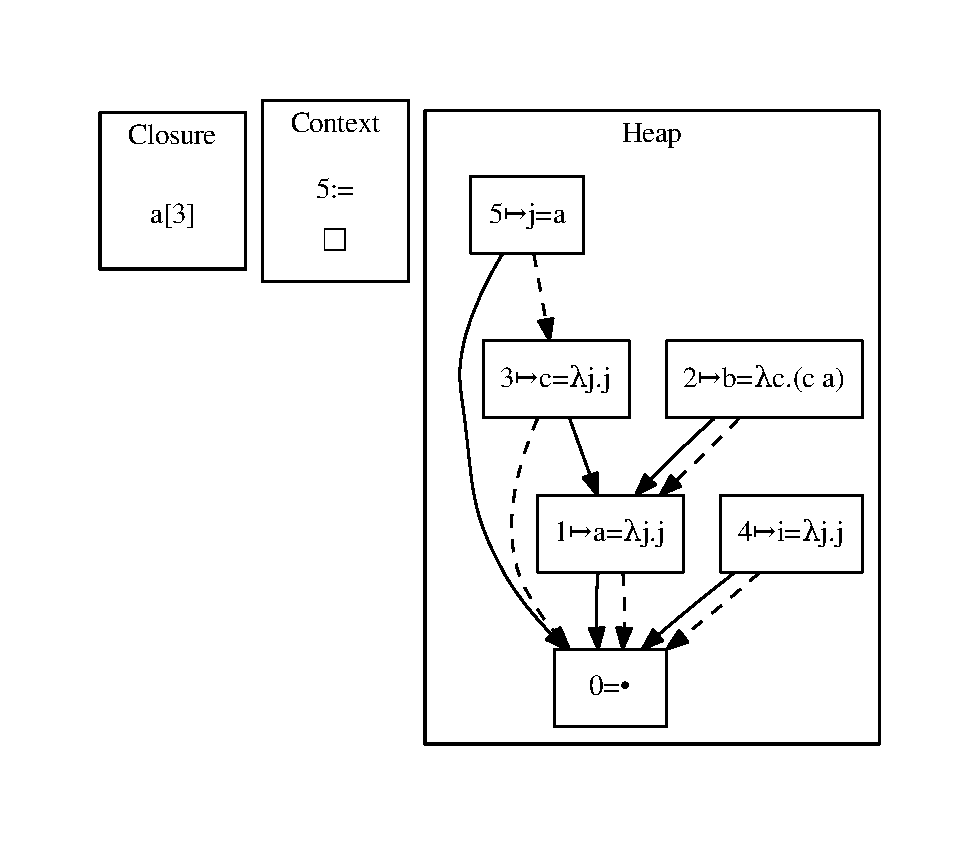
\includegraphics[width=\linewidth/3]{figures/20.pdf}
\caption{An example sequence of machine states during the evaluation of the term
$(\lambda a.(\lambda b.b \; a) (\lambda c.c
\; a)) ((\lambda i.i) (\lambda j.j))$. Order is left to right, top to bottom.
The free heap location $f$ is left out to save space. Dotted lines denote }
\label{fig:states}
\end{figure*}
